\subsection{Parametric Curves}
\todointern{add thing about control points in description and possibly names, because they're kinda important}
%As mentioned in the Introduction, the main challenge of our project is to convert the mesh based geometry, obtained on a previous step, back to CAD representation. 

To define NURBS from a mathematical standpoint, we first define so-called \emph{\Bez curves} and use them later for the definition of NURBS. 
\subsubsection{\Bez Curves}
A \Bez curve is a \textit{parametric} curve, which is often used for producing a smooth approximation of a given set of data points.
 
An analytical expression for the \Bez curve parametrized by the variable $u$ is given by:
\begin{equation*}
\vec{B}(u)=\sum\limits_{i=0}^n b_i^n(u) \vec{P}_i
\end{equation*}
where $\vec{P}_i$ is the $i^{\text{th}}$ control point, $i\in0,1, \dots ,n$ ($n+1$ control points in total), and
\begin{equation*}
b_i^n(u)=\binom{n}{i}(1-u)^{(n-i)}u^i
\end{equation*}
with $\binom{n}{i}$ being a binomial coefficient, is the $i^{\text{th}}$ \emph{Bernstein polynomial} (see \cite{lorentz2012bernstein}) of degree $n$.

In addition to the expression with the Bernstein polynomials, one can use a recursion formula (so-called \emph{de Casteljau Algorithm}) for the construction of the \Bez curve, which we will not cover here. 

Analogous to \Bez curves, one can also define a \textit{\Bez surface}. One of the ways of doing this, is by extending the set of control points indexed in one dimension, to a $2$-dimensional mesh of $n\times m$ control points $\vec{P}_{i,j}$, likewise extending the Bernstein polynomial basis to $2$D by taking the tensor product of it with itself. The resulting \textit{tensor product \Bez} (curve) \textit{surface} is then given by the analytical expression
\begin{equation*}
\vec{S}(u,v)=\sum\limits_{i=0}^n \sum\limits_{j=0}^m b_i^n(u) b_j^m(v) \vec{P}_{i,j}
\end{equation*}

\subsubsection{B-Splines and NURBS}
Extending the idea described in previous section, one could use \emph{B-spline basis functions} (see below) instead of the Bernstein polynomial basis.

Unlike with \Bez curves, for the B-splines a parameter domain is subdivided by so-called \textit{knots}. For the one-dimensional parameter domain $[u_{0}, u_{m}]$, the \textit{knot vector} will be given by $u_{0} \leq u_{1} \leq ... \leq u_{m}$. In most cases $u_{0} = 0, u_{m} = 1$ is chosen, so that we get the unit interval for our parameter values. For the case of NURBS, the knots $u_{0},..., u_{m}$ need not be equidistant -- hence the Non-Uniform in the beginning NU of NURBS.

Given a knot vector $[u_{0}, u_{m}]$ and a degree of B-spline $p$, the $i$-th B-spline basis function is then defined recursively as follows:
\begin{equation}
N_{i,0}(u) =  \begin{cases} 1, & \mbox{if } u_{i} \leq u < u_{i+1} \\ 0, & \mbox{otherwise } \end{cases}
\end{equation} 
\begin{equation}
N_{i,p}(u) = \frac{u - u_{i}}{u_{i+p} - u_{i}}N_{i, p-1}(u)  + \frac{u_{i+p+1}-u}{u_{i+p+1} - u_{i+1}}N_{i+1, p-1}(u)
\end{equation}
For $p=0$ we get just step functions, and $p=1$ familiar hat functions, whereas the quadratic basis functions look more complicated (\autoref{fig:bsplineBases}).
\begin{figure}
\centering
\begin{subfigure}[b]{.3\linewidth}
  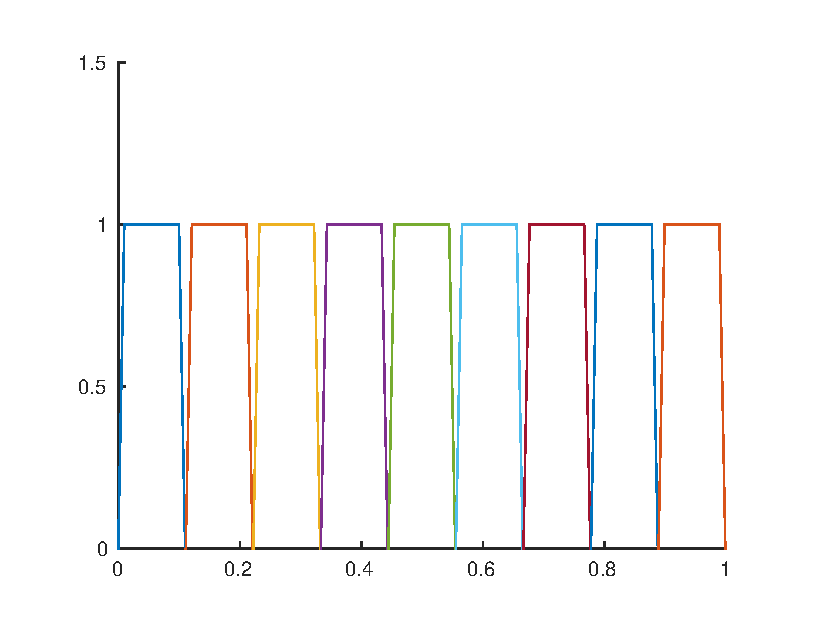
\includegraphics[width=\linewidth]{Pictures/basisconstant}
  \subcaption{B-spline basis for $p=0$}
  \label{fig:bspline_basis_constant}
\end{subfigure}%
\begin{subfigure}[b]{.3\linewidth}
  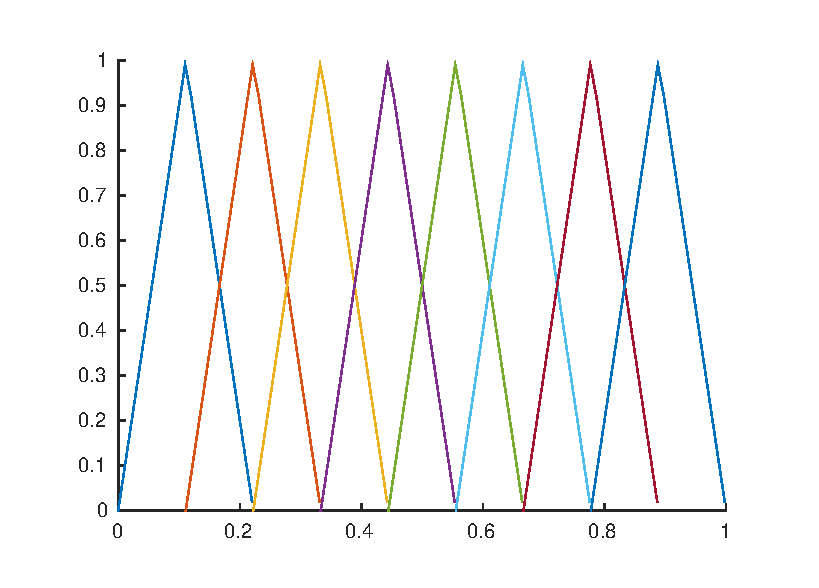
\includegraphics[width=\linewidth]{Pictures/basislinear}
  \subcaption{B-spline basis for $p=1$}
  \label{fig:bspline_basis_linear}
\end{subfigure}
\begin{subfigure}[b]{.3\linewidth}
  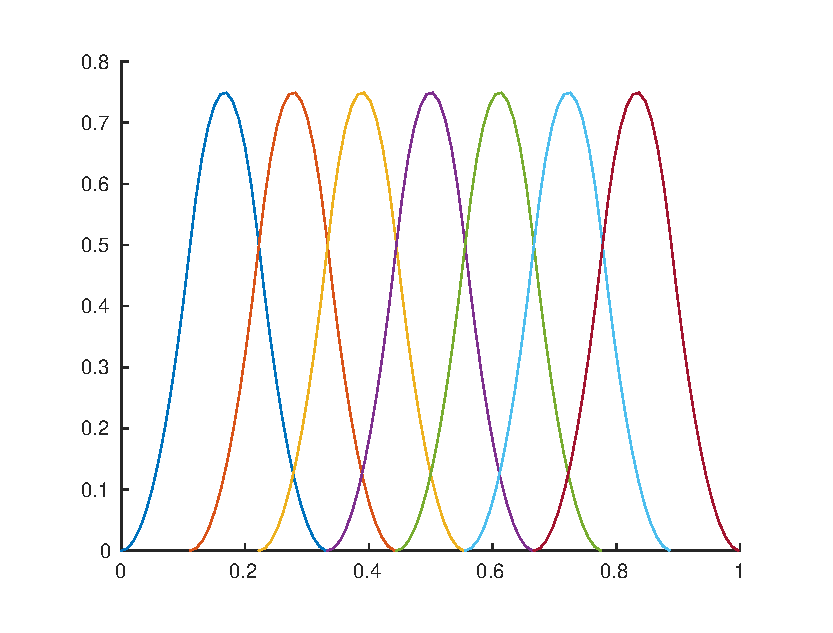
\includegraphics[width=\linewidth]{Pictures/basisquadratic}
  \subcaption{B-spline basis for $p=2$}
  \label{fig:lognorm_quadratic}
\end{subfigure}
\caption{B-spline basis functions, of degree $p=0$ (left), $p=1$ (middle) and $p=2$ (right).}
\label{fig:bsplineBases}
\end{figure}


By giving each of these basis functions a weight $\omega_i$ and normalizing them at each point by dividing by the total sum, we get the rational basis functions. Writing them out explicitly, in terms of B-spline basis functions $N_{i,p}$, the $n^{\text{th}}$-degree NURBS curve with $k$ control points $P_i$ is finally given by:
\begin{equation}
C(u) = \frac{\sum_{i=1}^{k}N_{i,n}\omega_{i}P_{i}}{\sum_{i=1}^{k}N_{i,n}\omega_{i}}.
\end{equation}

B-splines have the following properties, which are useful for our problem:
\begin{itemize}
\item Degree $n$ and number of control points $\vec{P}_{i\cdots m}$ are independent.
\item B-Splines only change locally (depending on the degree $n$) when a control point is changed.
\end{itemize}

Analogous to the tensor product \Bez curve surfaces, one can define tensor product B-spline or -NURBS surfaces. With varying degrees and number of control points, these can be made to fit a variety of shapes. However, as the parameters $u$ and $v$ define a square in their two-dimensional parameter domain, there is a limit to what topologies may be realized with just one such NURBS surface. For example, an open cylinder could be constructed by one such surface where one of the sides meets its own beginning, whereas something with multiple holes - like a double torus, or a non-flat 8-shaped surface, would be impossible. Therefore, when using NURBS, surfaces are most often modelled using a network of connected patches. \todointern{maybe should include an example picture here} For more information about NURBS see \cite{farin1999nurbs}.
